%██████╗ ███████╗███████╗██╗   ██╗██╗     ████████╗███████╗
%██╔══██╗██╔════╝██╔════╝██║   ██║██║     ╚══██╔══╝██╔════╝
%██████╔╝█████╗  ███████╗██║   ██║██║        ██║   ███████╗
%██╔══██╗██╔══╝  ╚════██║██║   ██║██║        ██║   ╚════██║
%██║  ██║███████╗███████║╚██████╔╝███████╗   ██║   ███████║
%╚═╝  ╚═╝╚══════╝╚══════╝ ╚═════╝ ╚══════╝   ╚═╝   ╚══════╝
%.:..:..:..:..:..:..:..:..:..:..:..:..:..:..:..:..:..:..:..:.
\chapter{Outcomes}

The OFDM system was modelled according to the IEEE 802.11 standard. \emph{One million} simulated bits were used to evaluate the system. A derivative variant was designated from the standard, having the following properties:
\begin{itemize}
	\item \emph{60} data sub-carriers.
	\item \emph{4} pilot sub-carriers.
	\item \emph{12} virtual sub-carriers.
	\item Cyclic extension of \emph{25\%} of symbol length.
	\item Guard interval of \emph{25\%}
\end{itemize}

 %___  ___  ___         ___                          
%| _ )| __|| _ \       / __| _  _  _ _ __ __ ___  ___
%| _ \| _| |   /      | (__ | || || '_|\ V // -_)(_-/
%|___/|___||_|_\       \___| \_._||_|   \_/ \___|/__/
%^*^^*^^*^^*^^*^^*^^*^^*^^*^^*^^*^^*^^*^^*^^*^^*^^*^^*^^*^^*^
%██████╗ ███████╗██████╗      ██████╗██╗   ██╗██████╗ ██╗   ██╗███████╗███████╗
%██╔══██╗██╔════╝██╔══██╗    ██╔════╝██║   ██║██╔══██╗██║   ██║██╔════╝██╔════╝
%██████╔╝█████╗  ██████╔╝    ██║     ██║   ██║██████╔╝██║   ██║█████╗  ███████╗
%██╔══██╗██╔══╝  ██╔══██╗    ██║     ██║   ██║██╔══██╗╚██╗ ██╔╝██╔══╝  ╚════██║
%██████╔╝███████╗██║  ██║    ╚██████╗╚██████╔╝██║  ██║ ╚████╔╝ ███████╗███████║
%╚═════╝ ╚══════╝╚═╝  ╚═╝     ╚═════╝ ╚═════╝ ╚═╝  ╚═╝  ╚═══╝  ╚══════╝╚══════╝
%.:..:..:..:..:..:..:..:..:..:..:..:..:..:..:..:..:..:..:..:.
\section{BER Curves}
The standard \gls{OFDM} was simulated to obtain its \gls{BER} performance curves over the three channel models \emph{(Rayleigh, Rician and AWGN.)} These were compared to the variant's.

\begin{figure}[!h]
	\centerline{\resizebox{!}{0.425\textheight}{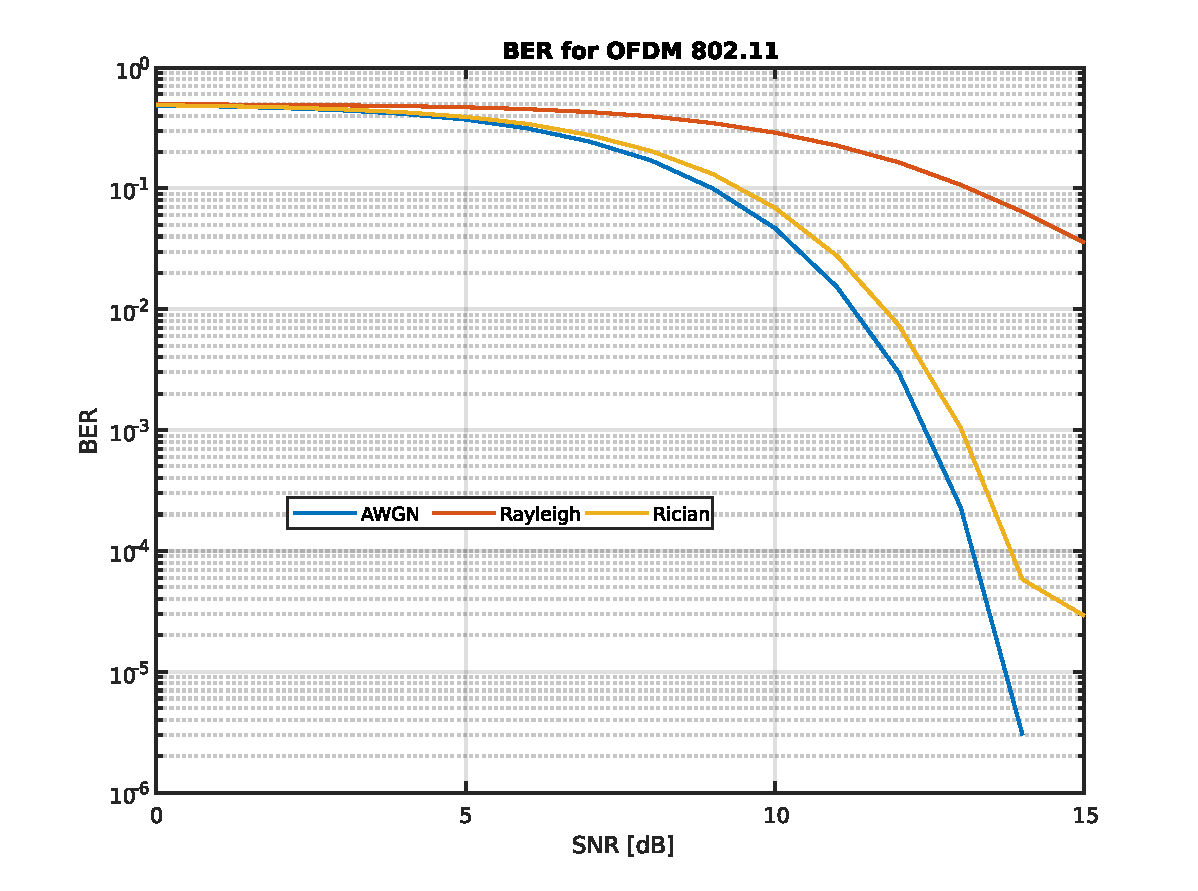
\includegraphics{Graphics/Results/combinedIEEE802.pdf}}}
	\caption{IEEE 802.11 BER Performance Curves}
	\label{res:fig:berstdCurves}
\end{figure}
\begin{figure}[!h]
	\centerline{\resizebox{!}{0.425\textheight}{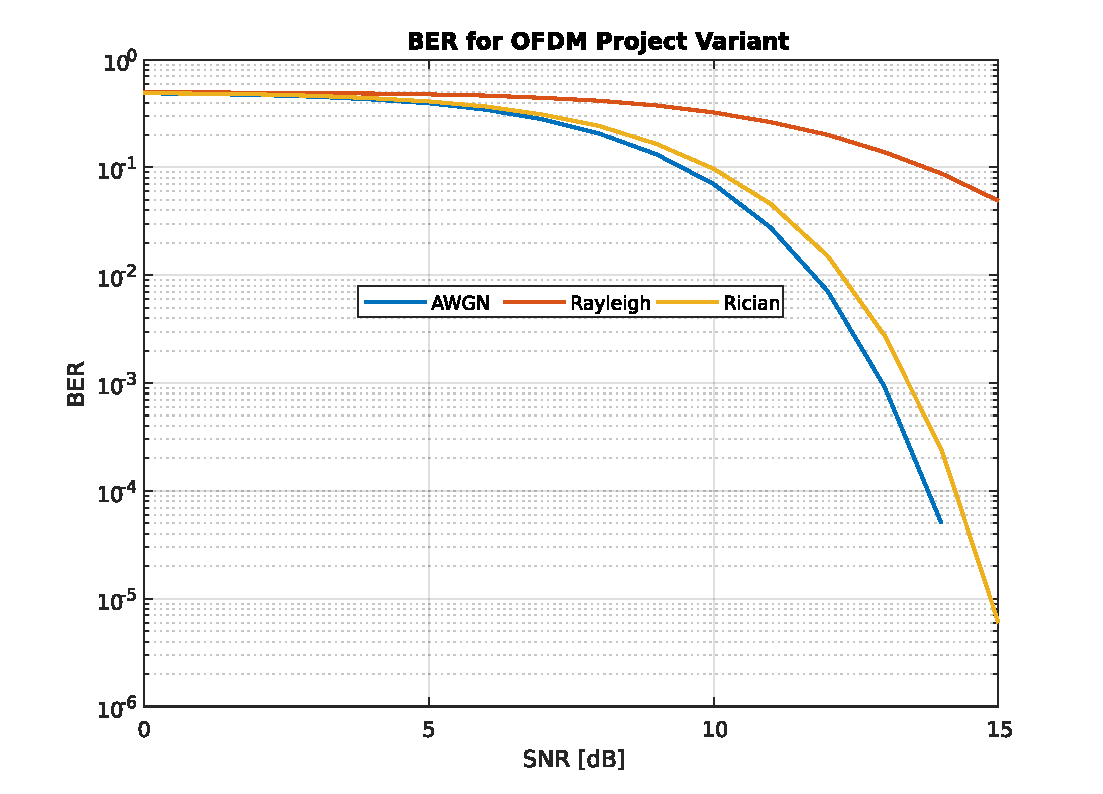
\includegraphics{Graphics/Results/combinedVariant.pdf}}}
	\caption{Project Variant BER Performance Curve}
	\label{res:fig:bervarCurves}
\end{figure}

\pagebreak


 %___  ___  ___  ___        _ __             __                                       
%| _ \/   \| _ \| _ \      | '_ \ ___  _ _  / _| ___  _ _  _ __   __ _  _ _   __  ___ 
%|  _/| - ||  _/|   /      | .__// -_)| '_||  _|/ _ \| '_|| '  \ / _` || ' \ / _|/ -_)
%|_|  |_|_||_|  |_|_\      |_|   \___||_|  |_|  \___/|_|  |_|_|_|\__/_||_||_|\__|\___|
%^*^^*^^*^^*^^*^^*^^*^^*^^*^^*^^*^^*^^*^^*^^*^^*^^*^^*^^*^^*^
%██████╗  █████╗ ██████╗ ██████╗ 
%██╔══██╗██╔══██╗██╔══██╗██╔══██╗
%██████╔╝███████║██████╔╝██████╔╝
%██╔═══╝ ██╔══██║██╔═══╝ ██╔══██╗
%██║     ██║  ██║██║     ██║  ██║
%╚═╝     ╚═╝  ╚═╝╚═╝     ╚═╝  ╚═╝
%.:..:..:..:..:..:..:..:..:..:..:..:..:..:..:..:..:..:..:..:.
\section{PAPR Performance}

The \gls{PAPR} was determined according to the definition stated in the literature review: the relation between maximum sample power in an OFDM symbol divided by the symbol's average power. For consistency, individual symbols' PAPRs were averaged to get each variant's equivalent value.

The values obtained are:
\begin{itemize}
	\item \emph{IEEE 802.11 } standard OFDM implementation: \SI{7.25}{\decibel}
	\item \emph{OFDM Variant} \SI{7.35}{\decibel}
\end{itemize}

The increase in average \gls{PAPR} from the standard OFDM implementation to the variant is expected since there are more data sub-carriers in the variant. This means that more signalling energy is expended in transmitting a symbol.
\pagebreak


  %___                             ___  _  _    _    _        __ _ 
 %/ __| _  _  _ _ __ __ ___       | __|(_)| |_ | |_ (_) _ _  / _` |
%| (__ | || || '_|\ V // -_)      | _| | ||  _||  _|| || ' \ \__. |
 %\___| \_._||_|   \_/ \___|      |_|  |_| \__| \__||_||_||_||___/ 
%^*^^*^^*^^*^^*^^*^^*^^*^^*^^*^^*^^*^^*^^*^^*^^*^^*^^*^^*^^*^
 %██████╗██╗   ██╗██████╗ ██╗   ██╗███████╗    ███████╗██╗████████╗████████╗██╗███╗   ██╗ ██████╗ 
%██╔════╝██║   ██║██╔══██╗██║   ██║██╔════╝    ██╔════╝██║╚══██╔══╝╚══██╔══╝██║████╗  ██║██╔════╝ 
%██║     ██║   ██║██████╔╝██║   ██║█████╗      █████╗  ██║   ██║      ██║   ██║██╔██╗ ██║██║  ███╗
%██║     ██║   ██║██╔══██╗╚██╗ ██╔╝██╔══╝      ██╔══╝  ██║   ██║      ██║   ██║██║╚██╗██║██║   ██║
%╚██████╗╚██████╔╝██║  ██║ ╚████╔╝ ███████╗    ██║     ██║   ██║      ██║   ██║██║ ╚████║╚██████╔╝
 %╚═════╝ ╚═════╝ ╚═╝  ╚═╝  ╚═══╝  ╚══════╝    ╚═╝     ╚═╝   ╚═╝      ╚═╝   ╚═╝╚═╝  ╚═══╝ ╚═════╝ 
%.:..:..:..:..:..:..:..:..:..:..:..:..:..:..:..:..:..:..:..:.
\section{Curve Fitting}

\subsection{Gaussian Channel Model}
The equation representing BER for the project's OFDM variant in a Gaussian channel is:
\begin{align*}
	y = f(x) &=
	\begin{cases}
		0.47Q \left(\frac{x - 7.5}{2.5}\right) & -\infty \leq x \leq 9.5 \\
		0.15Q \left(\frac{x - 10.5}{1.17}\right) & 9.5 < x \leq 15 \\
		0 & \text{otherwise}
	\end{cases}
\end{align*}
\begin{figure}[htpb!]
    \centering
    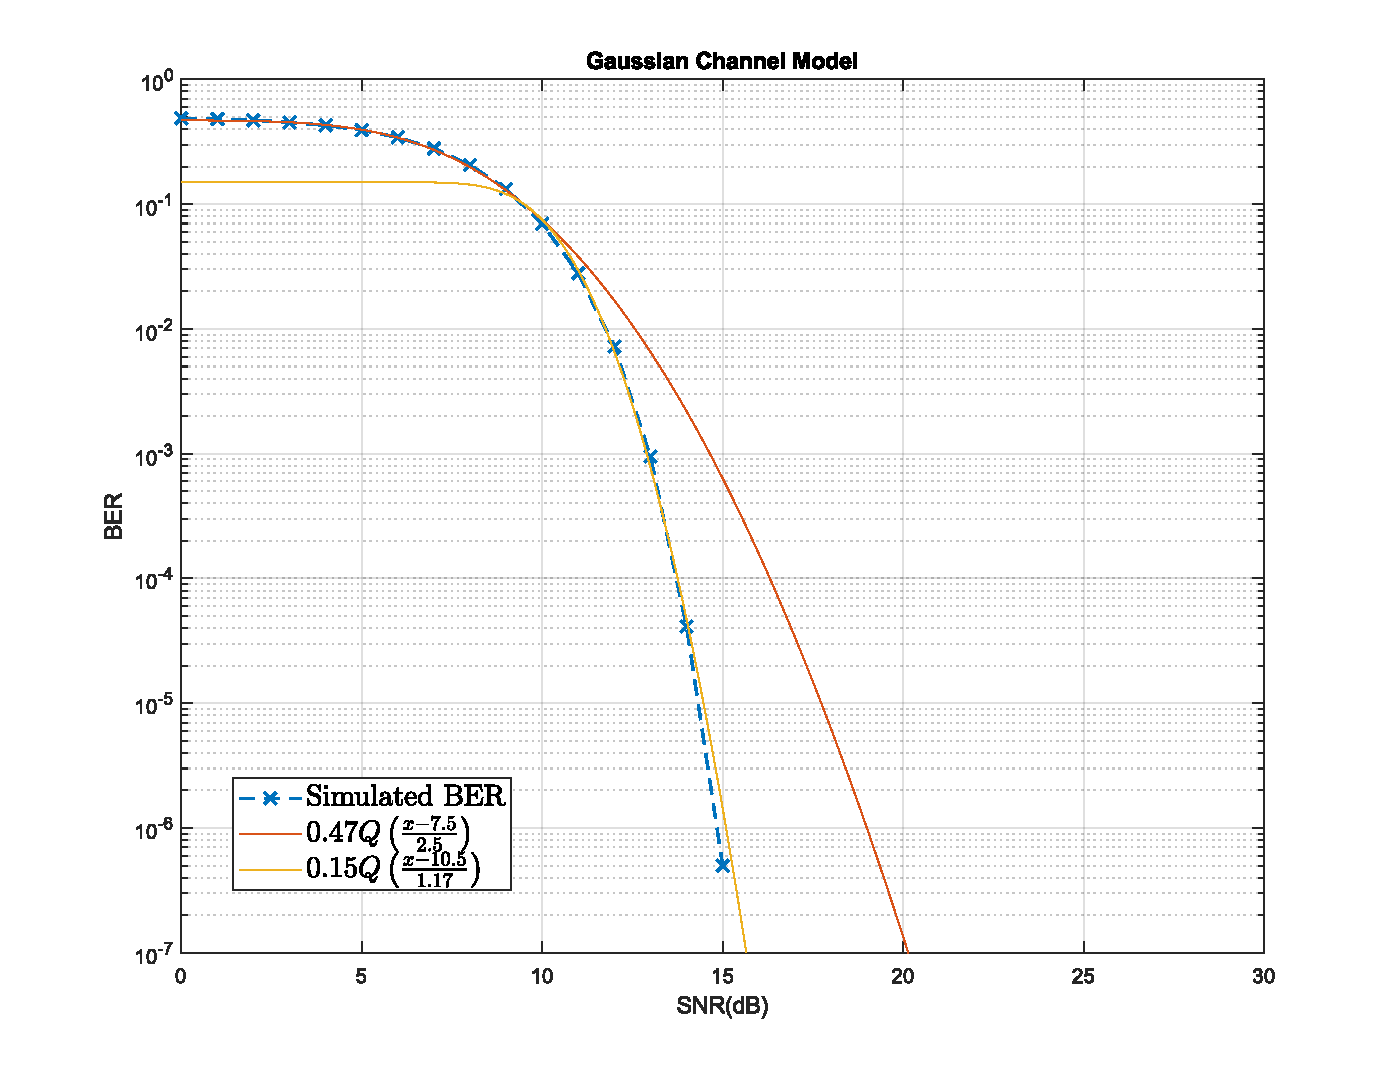
\includegraphics[scale=0.6]{Graphics/Methodology/GaussCurveFit.pdf}
    \caption{AWGN Channel curve fitting}
    \label{fig:gaussCurveFit}
\end{figure}
\pagebreak

\subsection{Rayleigh Channel Model}
The equation representing BER for the project's OFDM variant in a Rayleigh fading channel is:
\begin{align*}
	y = f(x) &=
	\begin{cases}
		0.5Q \left(\frac{x - 11.1}{3.05}\right) & -\infty \leq x \leq 17 \\
		1_E4Q \left(\frac{x - 35}{11}\right) & \text{otherwise} \\
		0 & \text{otherwise}
	\end{cases}
\end{align*}
\begin{figure}[htpb!]
    \centering
    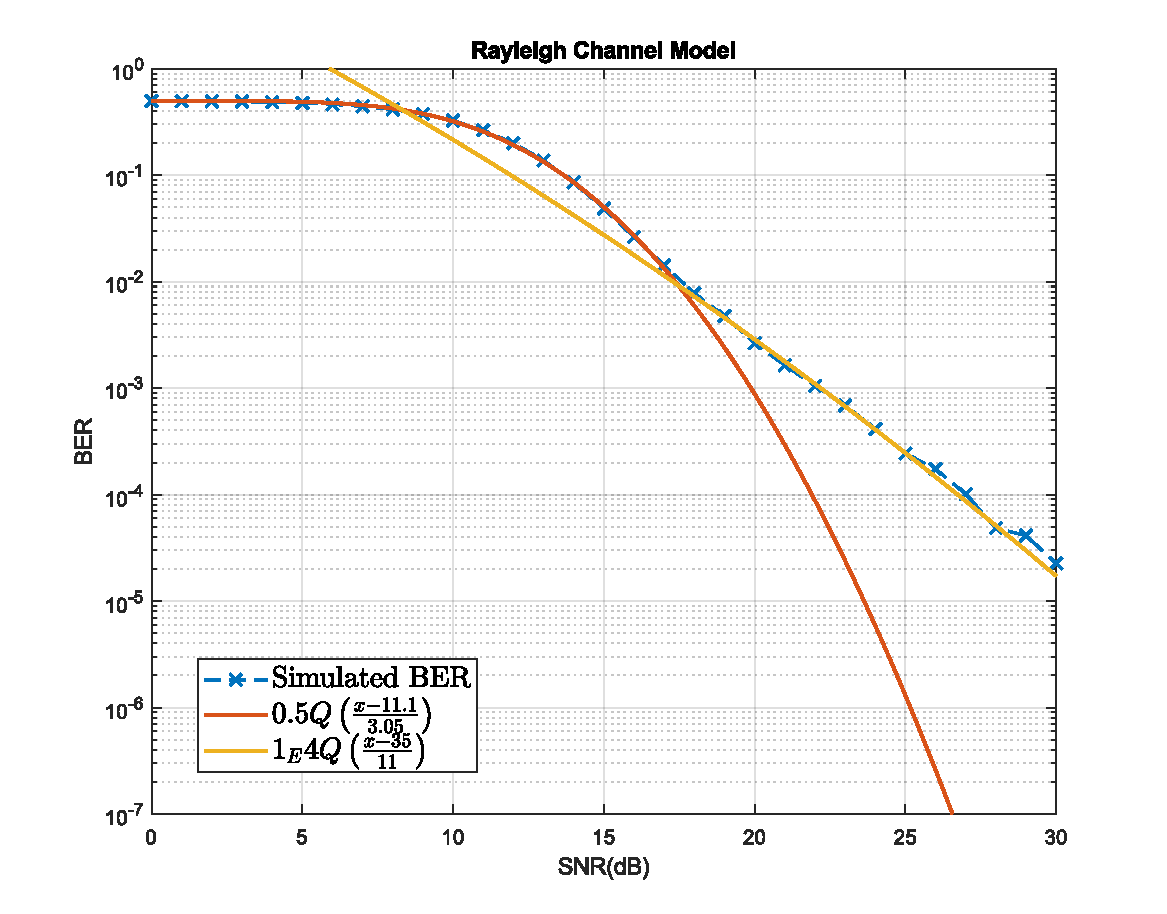
\includegraphics[scale=0.6]{Graphics/Methodology/RaylCurveFit.pdf}
    \caption{Rayleigh Channel Curve Fitting}
	\label{fig:raylCurveFit}
\end{figure}
\pagebreak

\subsection{Rician Channel Model}
The equation representing BER for the project's OFDM variant in a Rician fading channel is:
\begin{align}
	\label{res:RiceFn}
	y = f(x) &=
	\begin{cases}
		0.5 & -\infty < x \leq 0 \\
		aQ \left(\frac{x - b}{c}\right) & 0 < x \\
	\end{cases}
\end{align}
\begin{mathDef}
	\mathSymb{x}{\gls{SNR}}
	\mathSymb{a}{\[\begin{cases}0.004K^2 - 0.0081K + 0.4392 & 0 \leq K < 5 \\ 0.4 & 5 \leq K\end{cases}\]}
	\mathSymb{b}{-0.2895K + 11.222}
	\mathSymb{c}{-0.0917K + 2.785}
\end{mathDef}
The range of \(K\) for which equation \eqref{res:RiceFn} is valid is:
\[
	0 \leq K \leq 10.5
\]
\begin{figure}[htpb!]
    \centering
    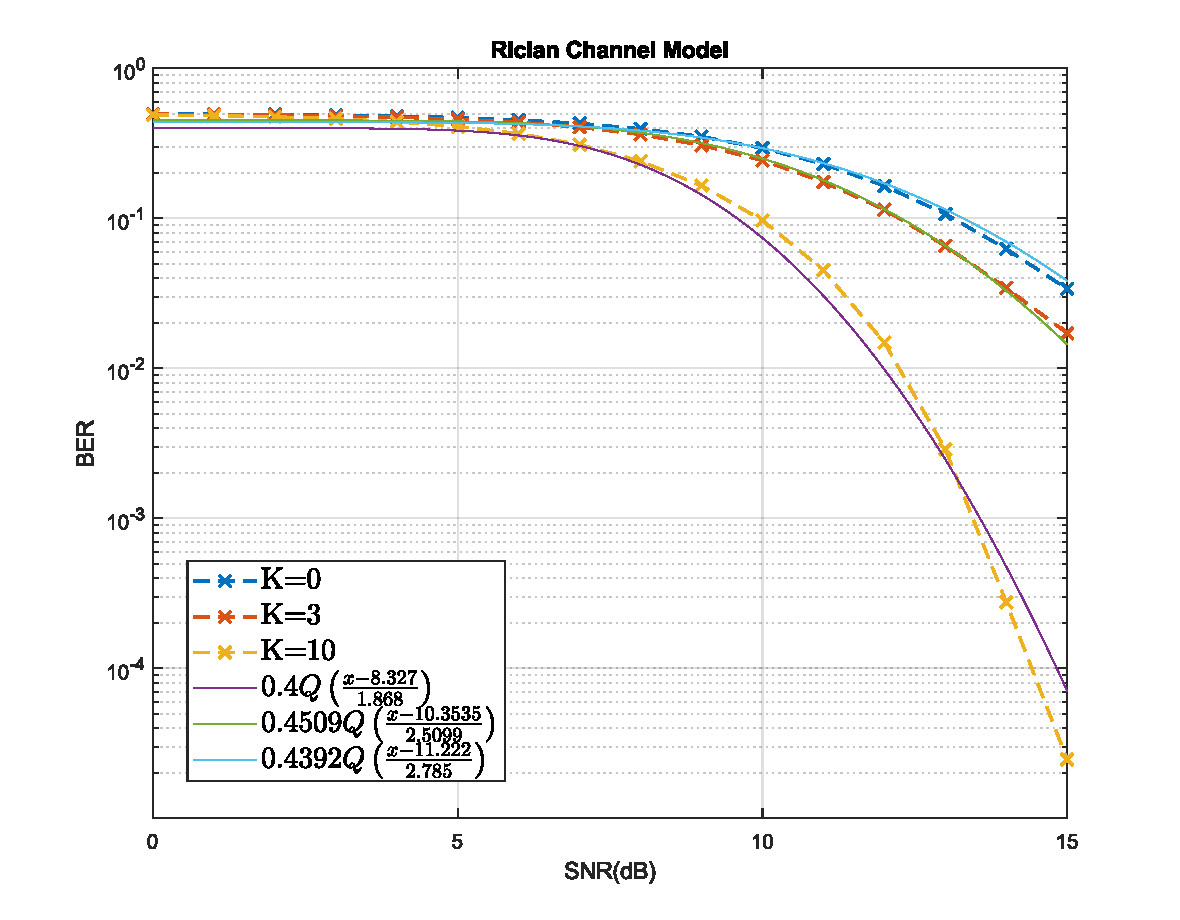
\includegraphics[scale=0.56]{Graphics/Methodology/RiceCurveFit.pdf}
    \caption{Rician Channel Curve Fitting}
	\label{fig:riceCurveFit}
\end{figure}


\pagebreak



